

\section{Results}\label{sec:results}

Starting with a sample of 2857 field RR Lyrae stars with both LINEAR and ZTF data, we found 228 stars exhibiting
convincing Blazhko effect. Out of these 228, 14 were selected via periodogram, and 214 via the scoring algorithm. 

From Fig.~\ref{fig:chi_final} we can see that most Blazhko stars selected via periodogram have very low $\chi^2_{dof}$ values for both 
LINEAR and ZTF data. Meanwhile, Blazhko stars selected via the scoring algorithm generally have low $\chi^2_{dof}$ LINEAR scores, with an average of 1.78, and higher $\chi^2_{dof}$ ZTF values,
with an average of 4.09. Most Blazhko stars are part of the 4-point $\chi^2_{dof}$ range (94 stars), with 66 stars in the 5-point range and 54 in the 3-point range. In accordance with this, the
average Blazhko candidate score is 5.90. Based on the light curve type, 78.95 \% of stars are RRab type, and 21.05 \% are RRc type stars. Ratio of RRab to RRc stars is in accordance with other works.

During visual analysis, we noticed that many Blazhko stars exhibited convincing Blazhko effect either in LINEAR or in ZTF data, with few examples of the effect in both datasets. 
Also, the modulation in light curves isn't constant for most stars, rather it varies throughout the observing season. In the following discussion we discuss how to utilize this finding.


\subsection{Statistical Properties of selected Blazhko Stars}

\begin{figure*}[ht]
    \centering
    \resizebox{\hsize}{!}{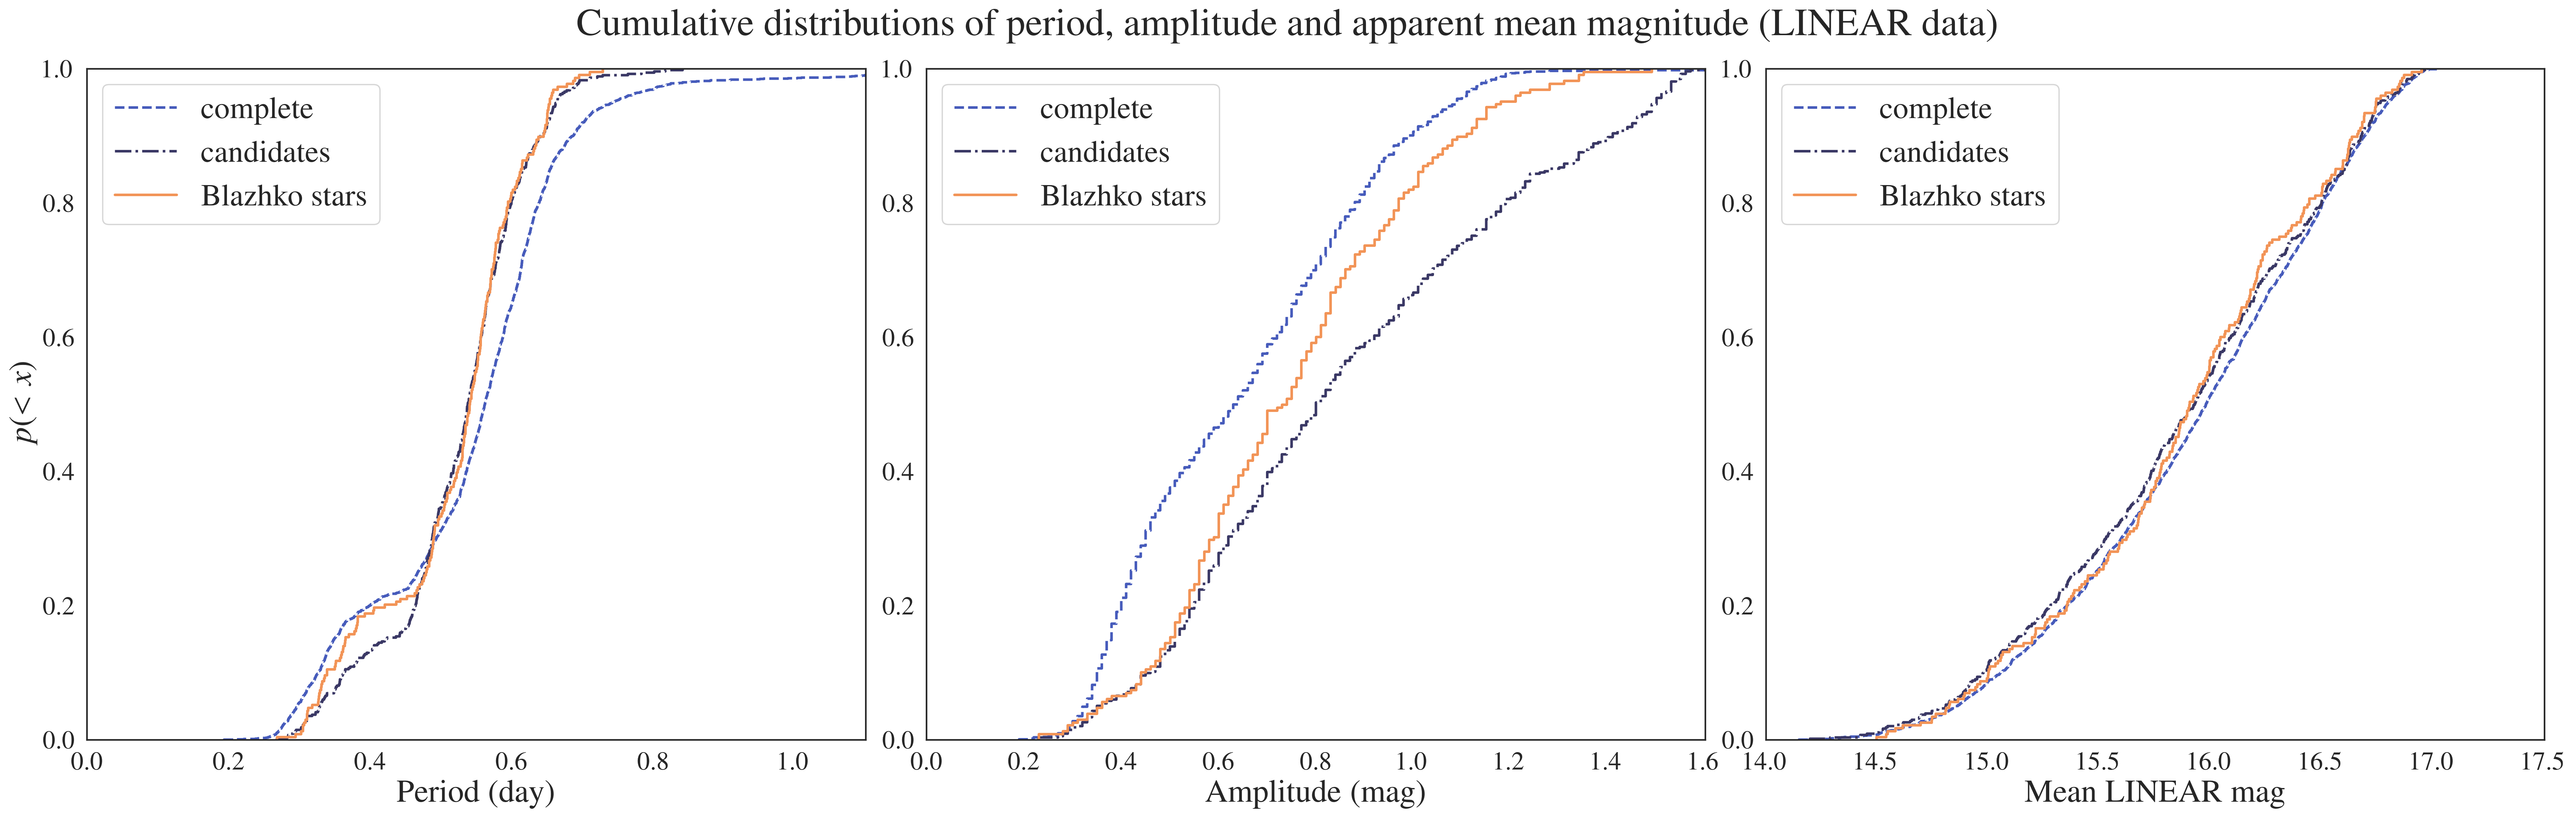
\includegraphics[width=16cm]{cumulative_distib_L.png}}
     \resizebox{\hsize}{!}{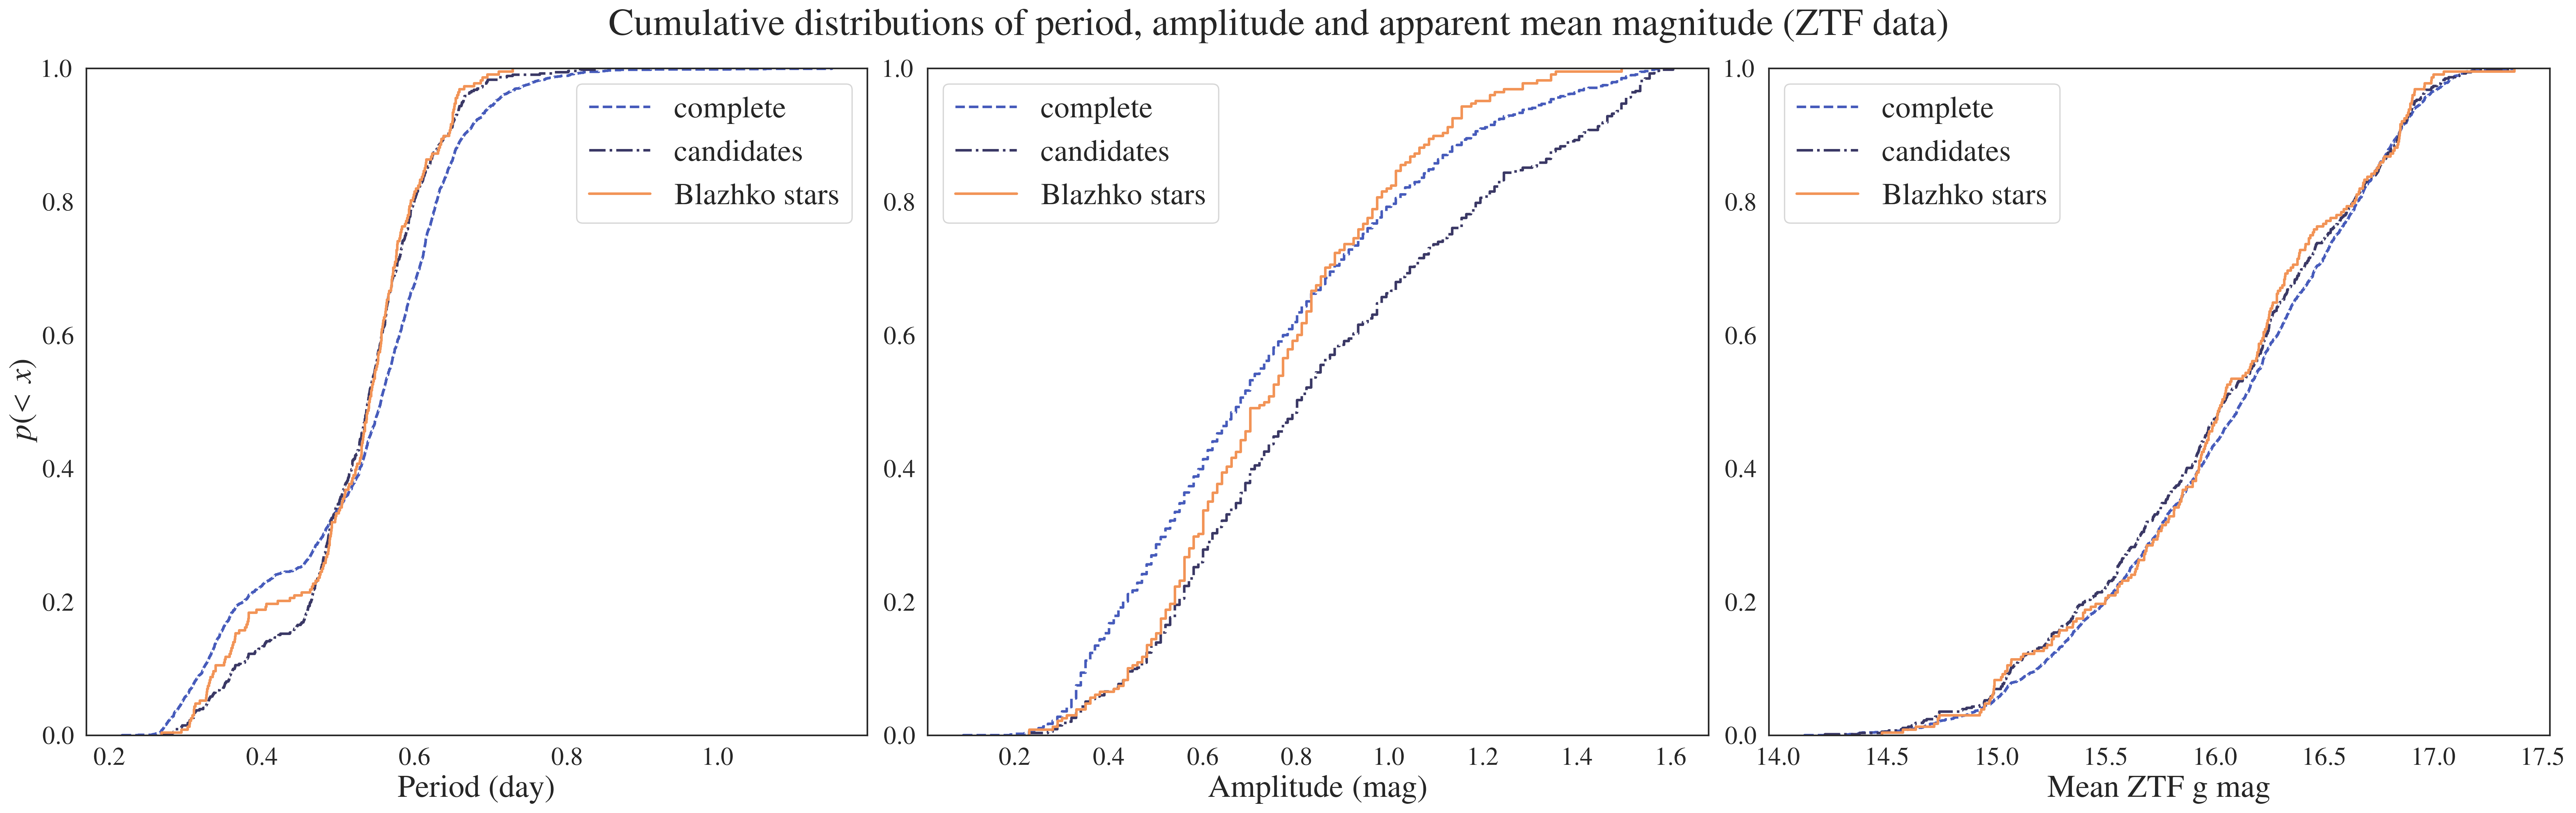
\includegraphics[width=16cm]{cumulative_distib.png}}
   \caption{A comparison of cumulative distributions of period (left),
   amplitude (middle) and apparent magnitude for starting sample,
   selected Blazhko candidates and visually verified Blazhko
   stars. The top row is based on LINEAR data and the bottom row is
   based on ZTF data. The differences in period and amplitude
   distributions are futher examined in figure~\ref{fig:AmplPeriod2D}.}
      \label{fig:AmplPeriod}
\end{figure*}

\begin{figure*}[ht]
    \centering
    \resizebox{\hsize}{!}{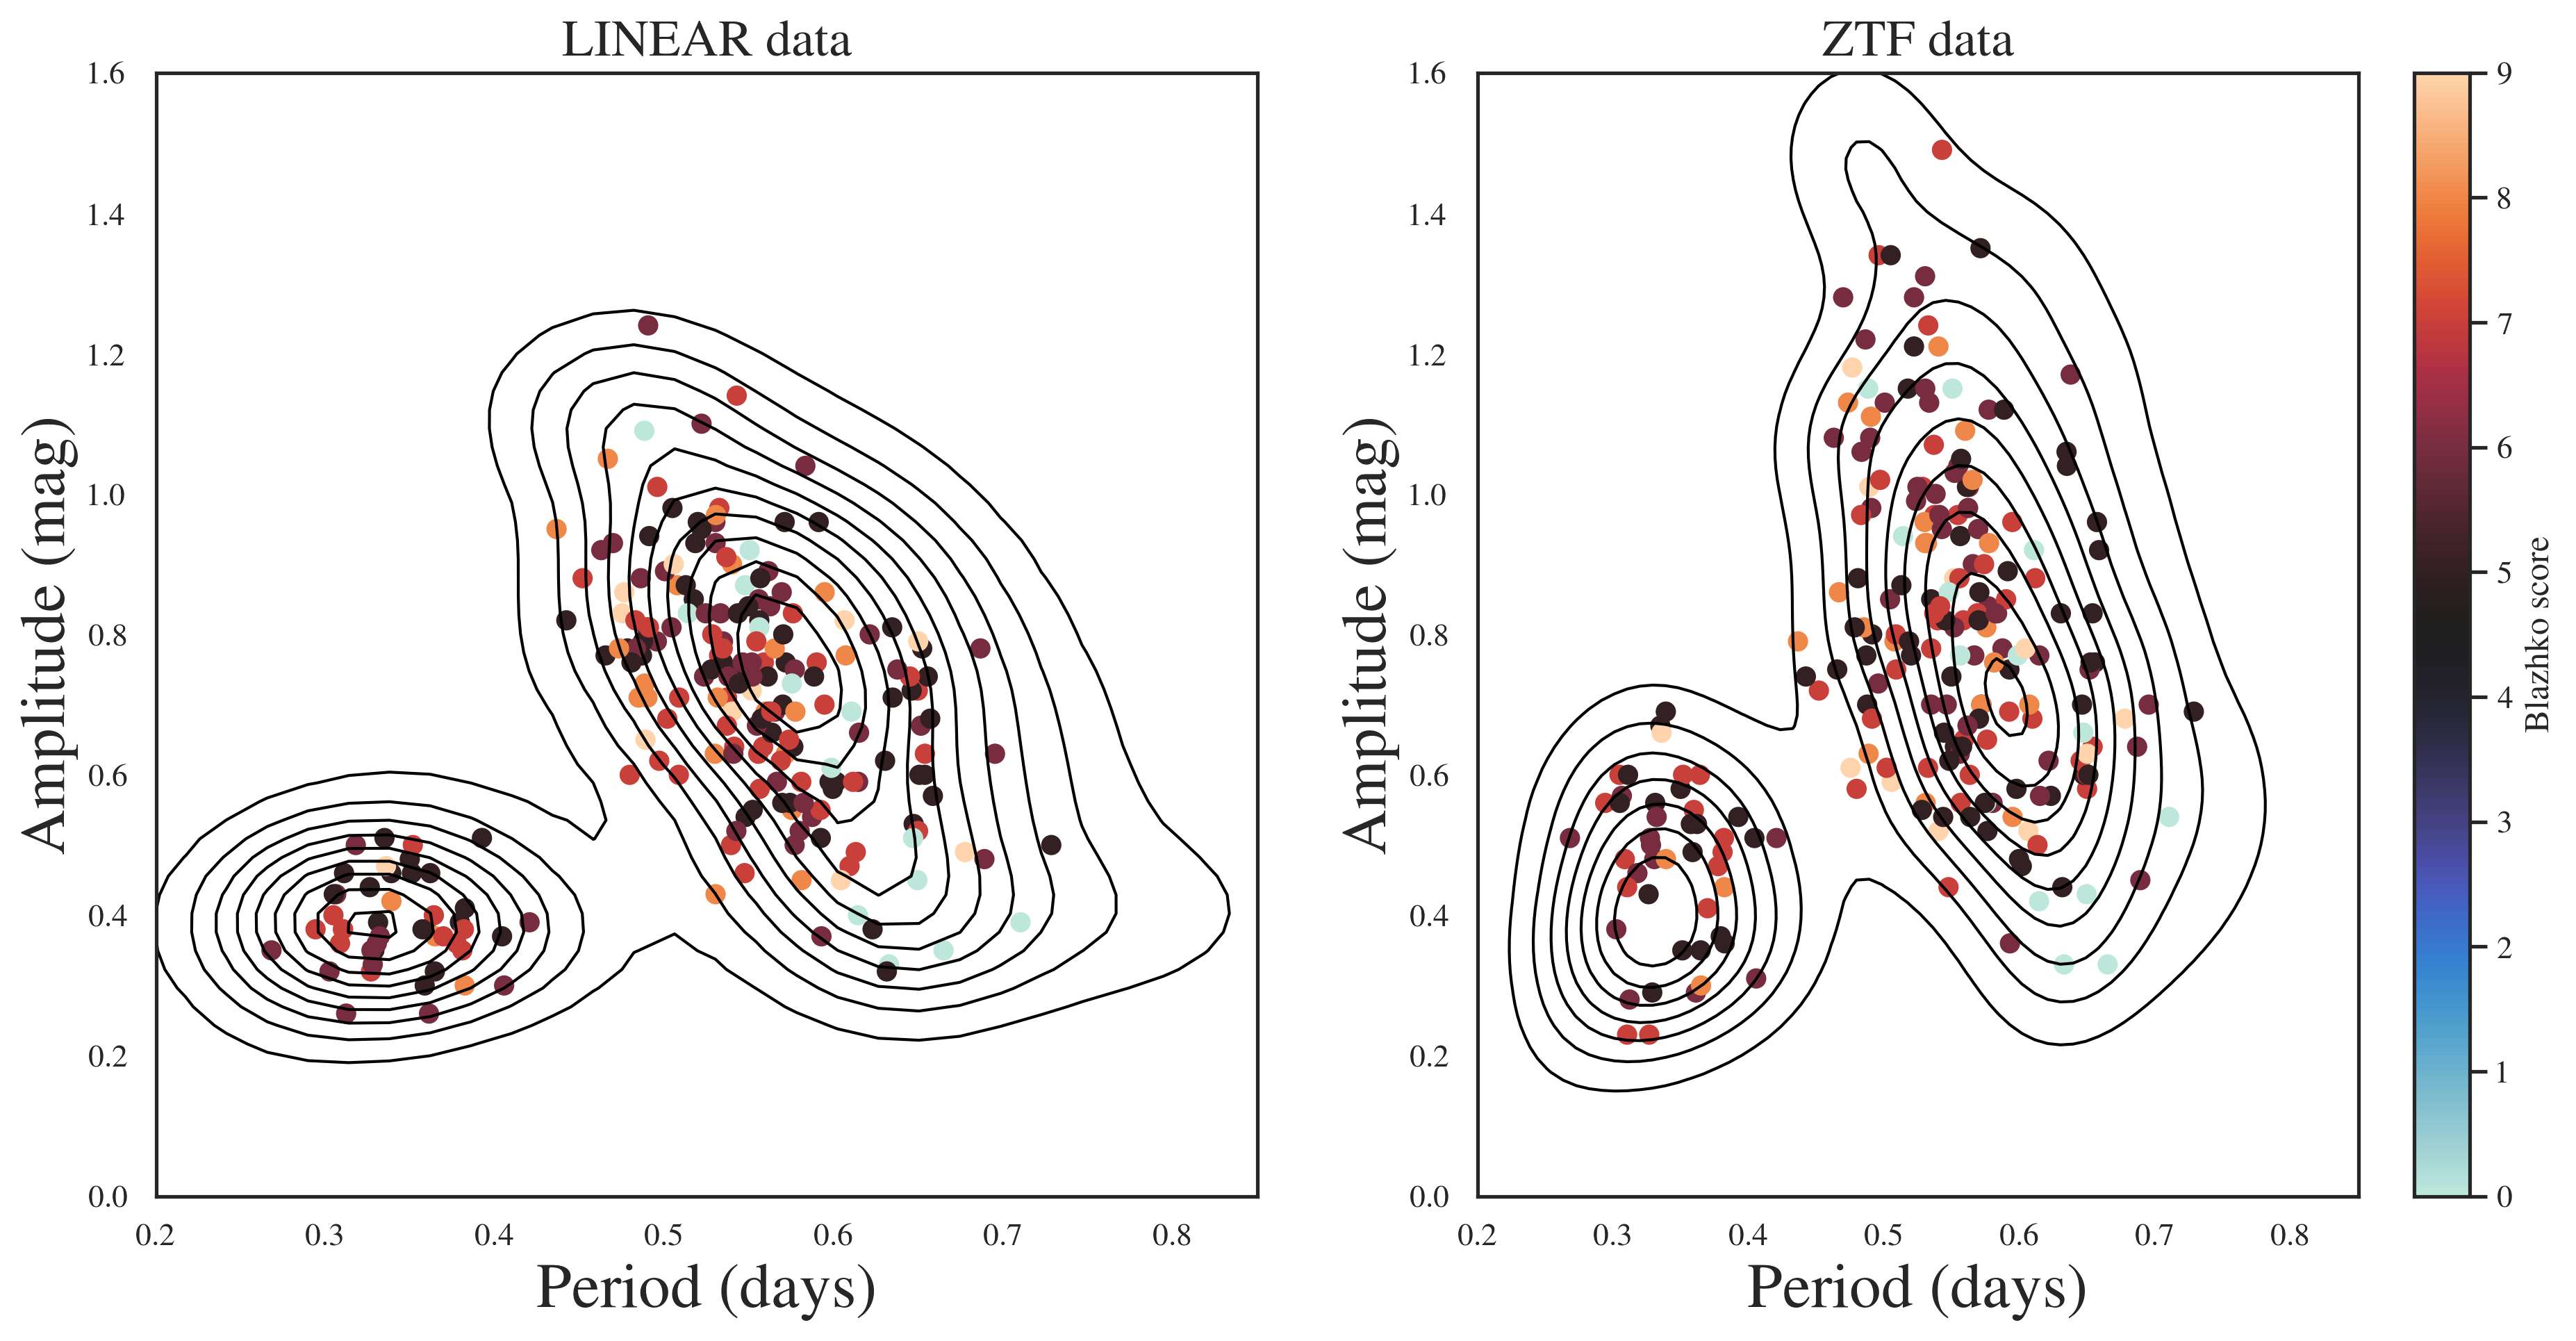
\includegraphics[width=16cm]{AmplPeriod.png}}
    \caption{Comparison of amplitude--period distributions (the Bailey
      diagram) for the starting sample of 1,996 RR Lyrae stars (contours)
        and 228 selected candidate Blazhko stars (symbols). The clump
        in the lower left corresponds to c type RR Lyrae and the
        other one to ab type. Note that the period distribution for ab
      type Blazhko stars is shifted left (by about 0.03 day, or 5\%).}
      \label{fig:AmplPeriod2D}
\end{figure*}


Marginal distributions of  period, amplitude and apparent magnitude
for starting sample and Blazhko stars are compared in Fig.~\ref{fig:AmplPeriod}. 

The median period for ab type Blazhko stars is 5\% shorter than for starting
RR Lyrae sample, while for c type Blazhko stars have 2\% longer median period. 

For the latter, the effect corresponds to only 1.1$\sigma$ deviation, while for ab type the
difference is significant at the 7.1$\sigma$ level. At the same time, the difference in
median amplitudes for ab type corresponds to only 0.6$\sigma$ deviation. 

Therefore, the only significantly detected difference is 5\% shorter periods for
ab type Blazhko stars, with an uncertainty of about 1\%. At a similar uncerainty level,
we don't detect period difference for c type stars, and don't detect any difference
in amplitude distribution. 


\subsection{Long-term behavior of Blazhko Stars}


There are stars where Blazhko effect is much more prominent in one survey than in other one,
strongly suggesting that Blazhko effect can appear and disappear on time scales shorter than
about a decade. Fig. XX shows a star (LINEARid = 23193507), where Blazhko effect is evident in LINEAR but not noticeable
in ZTF. Additional stars with similar behavior include LINEARid = 2889542, 3196780, 7723614, 8342007.
There are also stars where Blazhko effect is evident in ZTF but not in LINEAR data (e.g., LINEARid = 19466437, 14155360). 




